\section{Relationaler Datenbankentwurf}
\label{sec:abbildenRelational}

\textbf{Universalrelation}
\begin{items}
	\item \underline{Universalrelation} (von \( R_1, \dots, R_n \)): \( R = R_1 \bowtie \cdots \bowtie R_n \)
	\item \underline{Universalschlüssel}: Schlüssel der Universalrelation
	\item Beispiel: \( R_1, R_2, R_3 \):
	\begin{figure}[H]\centering\label{NonJoin}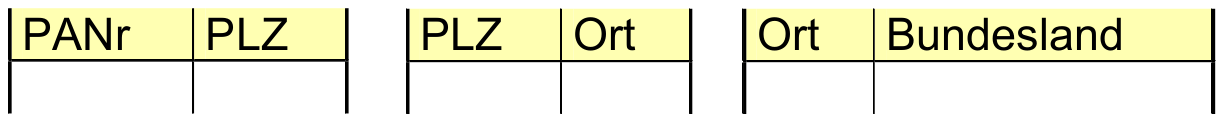
\includegraphics[width=0.33\textwidth]{NonJoin}\end{figure}
	\item \quad \( R_1 \bowtie R_2 \bowtie R_3 \):
	\begin{figure}[H]\centering\label{Join}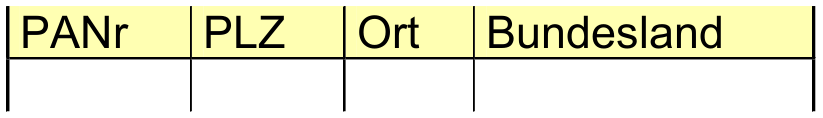
\includegraphics[width=0.33\textwidth]{Join}\end{figure}
\end{items}

\textbf{Funktionale Relation}
\begin{items}
	\item In Relation \( R(X,Y) \) ist \( Y \) von \( X \) funktional abhängig (schreibe \( X \to Y \)), falls zu jedem \( X \)-Wert genau ein \( Y \)-Wert gehört (z.B. Buchtitel, ISBN-Nummer oder Stadt, Bundesland)
	\item \( \leadsto \) ``\( X \) bestimmt \( Y \)''
	\item \( F \): Menge von FDs (\emph{funcional dependencies}), \( f \in F \) einzelne FD
	\item \( F \) impliziert \( f \): \( F |= f \)
	\item \underline{Hülle}: \( F_R^+ = \{ f \mid (f \text{ FD über} R) \wedge F |= f \} \)
	\item \underline{Transitiv}: PLZ \( \to \) Ort \( \to \) Bundesland \\* \( \leadsto \) PLZ \( \to \) Bundesland
	\item \underline{Projektiv}: ISBN \( \to \) Autor Verlag \\* \( \leadsto \) ISBN \( \to \) Autor
	\item \underline{Akkumulativ}: ISBN \( \to \) Verlag Autor, Autor \( \to \) Straße Ort \\* \( \leadsto \) ISBN \( \to \) Verlag Autor Straße
	\item Äquivalente FD-Mengen (Überdeckungen): \( F \equiv G \) falls \( F^+ = G^+ \)
\end{items}

\textbf{Anomalien}
\begin{figure}[H]\centering\label{Anomalien}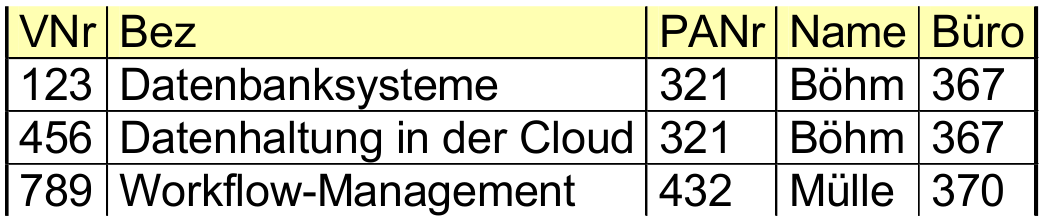
\includegraphics[width=0.33\textwidth]{Anomalien}\end{figure}
\begin{items}
	\item \underline{Updateanomalie}: Büro von Böhm ändert sich \\* \( \leadsto \) Änderung mehrerer Einträge \\* \( \leadsto \) Aufwendig, fehleranfällig. Wie vermeiden?
	\item \underline{Einfügeanomalie}: Neuer Dozent ohne VL (NULL-Werte) \\* \( \leadsto \) Was wenn VNr Schlüssel?
	\item \underline{Löschanomalie}: Mülle hält Workflow nicht mehr \\* \( \leadsto \) Tupel löschen \( \leadsto \) Müssel-Information verloren
\end{items}

\textbf{Abhängigkeitstreue}
\begin{items}
	\item Beispiel: (InvNr, Titel, \underline{ISBN}, \underline{Autor}) \\* oder (InvNr, Titel, \underline{ISBN}), (\underline{ISBN}, \underline{Autor}) \\* oder (InvNr, Titel, \underline{ISBN}), (\underline{ISBN}, Autor)?	
	\item Abhängigkeitstreu: Alle gegebenen Abhängigkeiten sind durch Schlüssel repräsentiert
\end{items}

\textbf{Verbundtreue}
\begin{items}
	\item Originalrelationen können durch Verbund der Basisrelationen wiedergewonnen werden
\end{items}

\newpage

\textbf{Entwurfsziel}
\begin{items}
	\item Relationenschemata, (Fremd-)Sclüssel so wählen, dass
	\begin{enumeration}
		\item alle Anwendungsdaten aus Basisrelation hergeleitet werden können (\emph{Verbundtruee})
		\item nur semantisch sinnvolle und konsistente Anwendungsdaten dargestellt werden können (\emph{Abhängigkeitstreue})
		\item möglichst nicht-redundante Daten
	\end{enumeration}
\end{items}

\textbf{Erste Normalform}
\begin{items}
	\item Nur atomare Attribute in Relationenschemata
\end{items}

\textbf{Zweite Normalform}
\begin{items}
	\item \underline{Volle FD}: \( \beta \) ist voll funktional abhängig von \( \alpha \), wenn aus \( \alpha \) kein Attribut entfernt werden kann, so dass FD immer noch gilt.
	\item Gegenbeispiel: PLZ, Bundesland \( \to \) Ort
	\item \underline{Partielle FD}: liegt vor, wenn ein Nicht-Primattribut voll funktional von einem Teil eines Schlüsselkandidaten abhängt
	\item \underline{Zweite NF}: keine partiellen Abhängigkeiten \\* \( \leadsto \) Durch Struktur der Abhöngigkeiten Redundanzen entdecken
\end{items}

\textbf{Dritte Normalform}
\begin{items}
	\item \underline{Transitive Abhängigkeit}: Schlüssel \( K \) bestimmt Attributmenge \( X \) funktional, ist selber aber auch Attributmenge \( Y \) \\* \( \leadsto \) transitive Abhängigkeit \(  \to X \to Y \)
	\item \underline{dritte NF}: Keine transitiven Abhängigkeiten zwischen einem möglichen Schlüssel und weiteren nicht-Primattributen
	\item Erreichen durch Elimination von \( Y \) und Kopie von \( X \)
	\item 3NF impliziert 2NF, da partielle Abhängigkeit Spezialfall von transitiver Abhängigkeit
\end{items}

\textbf{Boyce-Codd-Normalform}
\begin{items}
	\item Relationenschema \( \mathcal{R} \) mit FDs \( F \) ist in BCNF, wenn für jede FD \( \alpha \to \beta \) eine der folgenden Bedingungen gilt:
	\begin{enumeration}
		\item \( \beta \subseteq \alpha \) (triviale Abhängigkeit)
		\item \( \alpha \) Schlüssel von \( \mathcal{R} \) (oder Obermege eines Schlüssels von \( \mathcal{RLÖ} \))
	\end{enumeration}
	\item liefert Zerlegung von \( \mathcal{R}_i \) in \( \mathcal{R}_{i1} = (\alpha \cup \beta), \mathcal{R}_{i2} = \mathcal{R}_i-(\alpha \cup \beta) \) \\* (\( F \ni f : \alpha \to \beta, \beta \) maximal)
\end{items}

\textbf{Minimalität}
\begin{items}
	\item Ziel: Kiterien mit möglichst wenigen Relationenschemata erreichen
\end{items}

\textbf{Dekomposition}
\begin{items}
	\item Prinzip: Immer wenn \( X \to Y \to Z \) wird Relation zerlegt
	\item erreicht nur 3NF und Verbundtreue
	\item \underline{Normalisierung}: Falls \( K \to X \to Y \), dann \( Y \) aus \( R \) entfernen und mit \( X \) in neues Relationenschema stecken
	\item Beispiel: \( U = \{ \text{PANr}, \text{PLZ}, \text{Ort}, \text{Land}, \text{Staat} \} \), \\*
	\( F = \{ \text{PANr} \to \text{PLZ}, \text{PLZ} \to \text{Ort}, \text{Ort} \to \text{Land}, \text{Land} \to \text{Staat} \} \) \\*
	\( \leadsto \) \( (U,K(F)) = (\{ \text{PANr}, \text{PLZ}, \text{Ort}, \text{Land}, \text{Staat} \}, \{ \{ \text{PANr} \} \}) \) \\*
	Betrachte \( \text{PANr} \to \text{Land} \to \text{Staat} \). Neue Relationen:
	\begin{enumeration}
		\item \( R_1 = \{ \text{Land}, \text{Staat} \} \)
		\item \( R_2 = \{ \text{PANr}, \text{PLZ}, \text{Ort}, \text{Land} \} \)
	\end{enumeration}
	Wiederholen mit \( R_2 \)
	\item \underline{Vorteile}: 3NF, Verbundtreue
	\item \underline{Nachteile}: Keine Abhängigkeitstreue, keine Minimalität, reihenfolgeabhängig, NP-vollständig (Schlüsselsuche)
\end{items}

\newpage

\textbf{Syntheseverfahren}
\begin{items}
	\item Prinzip: Synthese formt Original-FD-Menge \( F \) in Menge von Schlüsselabhängigkeiten \( G \) so um, dass \( F \equiv G \)
	\item Abhängigkeitstreue integriert
	\item 3NF und Minimalität werden reihenfolgeunabhängig erreicht
	\item polynomielle Zeitkomplexität
	\item Übersicht:
	\begin{enumeration}
		\item Redundanzen eliminieren: \\*
		Entfernen unnötiger FDs und Attribute (\( f \) überflüssig wenn \( F \equiv F - \{  f \} \), überflüssige Attribute später)
		\item FDs zu Äquivalenzklassen zusammenfassen: \\*
		FDs in selber Klasse, wenn sie äquivalente linke Seiten haben \( \leadsto \) ein Relationenschema pro Äquivalenzklasse
	\end{enumeration}
	\item Beispiel: \( F = \{ A \to B, AB \to C, A \to C, B \to A, C \to E \} \)
	\begin{enumeration}
		\item Redundante FDs: \( A \to C \) \\* Stand: \( F' = \{ A \to B, AB \to C, B \to A, C \to E \} \)
		\item Überflüssige Attribute: \( B \) in \( AB \to C \) \\* Stand: \( F'' = \{ \underbrace{A \to B, A \to C, B \to A}_{\text{Äquivalenzklasse}}, C \to E \} \)
		\item Ergebnis Relationenschema: \\* \( (ABC, \{ \{ A \}, \{ B \} \}), (CE, \{ \{ C \} \}) \)
	\end{enumeration}
\end{items}

\textbf{Mehrwertige Abhängigkeiten}
\begin{items}
	\item \underline{Mehrwertige Abhängigkeit} (\emph{multi value dependency, MVD}): \\*
		Jeder Wert des abhängigen Attributes kommt in Kombination mit allen Werten der anderen Attribute vor
	\item Redundanzbehaftet
	\item Beispiel:
	\begin{center}
		\begin{tabular}{|lll|}
		  \hline
		  \textbf{Kurs} & \textbf{Buch} & \textbf{Dozent} \\
		  \hline
		  AHA & Silberschatz & John D \\
		  AHA & Nederpelt & John D \\
		  AHA & Silberschatz & William M \\
		  AHA & Nederpelt & William M \\
		  \hline
		\end{tabular}
	\end{center}
	Neues Buch: für jeden Dozenten anlegen \( \leadsto \) MVD
\end{items}

\textbf{Vierte Normalform}
\begin{items}
	\item Beispiel: Relation mit Attributen \emph{Name}, \emph{Neffe}, \emph{Hobby} \\*
		Es gelte MVD: \emph{Name} \( \twoheadrightarrow \) Neffe \\*
		Wenn \\*
		(Heinrich, Martin, Autos) und (Heinrich, Thomas, Basteln) \\*
		\( \in r \), dann auch \\*
		(Heinrich, Martin, Basteln) und (Heinrich, Thomas, Autos)
	\item Formal: \( r \) genügt MVD \( X \twoheadrightarrow Y \Leftrightarrow \) \\*
		\( \forall t_1, t_2 \in r: [(t_1 \neq t_2 \wedge t_1(X) = t_2(X)) \\* \Rightarrow \exists t_3 \in r: t_3(X)=t_1(X) \wedge t_3(Y)=t_1(Y) \wedge t_3(Z) = t_2(Z) ] \) 
	\item 4NF: solche MVDs aufspalten
	\item Trivial, wenn keine weiteren Attribute im zugehörigen Schema
\end{items}

\begin{fragen}
	\begin{enumeration}
		\item Erläutern Sie die folgenden Begriffe: Redundanz, Funktionale Abhängigkeit, Normalform, Verbundtreue, Abhängigkeitstreue, Minimalität.
		\item Erläutern Sie die Aussage: ``Funktionale Abhängigkeiten beinhalten semantische Informationen.''
		\item Welche Anomalien kennen Sie? Erläutern Sie für jede dieser Anomalien, warum Sie störend ist.
		\item Warum braucht man für Verbundtreue Kriterien, für Abhängigkeitstreue jedoch scheinbar nicht?
		\item Welche Normalformen kennen Sie? Sagen Sie umgangssprachlich, wie sie definiert sind.
	\end{enumeration}
\end{fragen}